\documentclass[a4]{article}
\usepackage{gnuplottex}
\usepackage{csvsimple}
\usepackage{subcaption}
\usepackage{amsmath}
\usepackage{graphicx}
\usepackage{epstopdf}
\usepackage{float}

\graphicspath{ {./image/} }

\title{COMP26120 Lab 3 Report}
\author{Ziyi Li}
\begin{document}
\maketitle

\section{Experiment 1}

In this experiment, I use mode 4 in my program. The hash value of a string is calculated by:
$$ h(s) = (a * sum + b) \  mod \  s.length$$
where s is a string, and a,b,sum are calculated by:
$$ a(s) = ord(s[0])^2$$
$$ b(s) = ord(s[-1])^3$$
$$ sum(s) = \sum^{s.length}_{i=0}(ord(s[i])^3)$$


\subsection{Hypothesis}

Any distinct string would get a unique hash value that represents its coordinate in the array. 
So the complexity of both insert and search is O(1)
\\ \hspace*{\fill} \\
\noindent This is the ideal situation, when the size of HashSet is enough, every element will have a unique hash value. When inserting the data, it can always find a free place(unoccupied) place and store it. It is the same with search, the program calculates the hash value of the data and finds the data in the place of that value directly. However, in real situations, it is possible that collisions happen, which means the place of that value should be has been occupied. So we need to apply the store procedure with collision, which is to search after that index linearly until finding a free place. When the pointer reached the end of the array, jump back to the start. 
I already applied occupation rate detection of the whole set, when the rate is larger than 0.5, resize will be applied, so it is not possible that the array is full.

\subsection{Design}

Python Jupyter notebook is used to test the hypothesis. The test file is in python hashset\_report.ipynb

\noindent Initial size of HashSet is (length of test file / 0.5).

\noindent The test data is a list containing N random strings (word length is 10).

\noindent Tests will insert all words and then search all words. The hit rate is 100\% which means there will be no failure when searching.

\noindent The size of the test set starts from 100 and ends with 100000, the step is 100.



\subsection{Results}

The result is in file hashset\_mode4\_result.csv

Definition:

Avg insert - The average step of finding address to insert element

Avg find - The average step of finding address and compare with element

Collision rate - Total collision number divides hashset size
\\
\noindent Charts are in the next page.

\begin{figure}[H]
    \begin{minipage}{0.48\textwidth}
    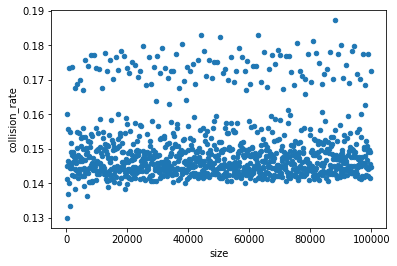
\includegraphics[width=0.95\textwidth]{h-size-collision.png}
    \caption{Size - Collision rate}
    \end{minipage}
    \begin{minipage}{0.48\textwidth}
    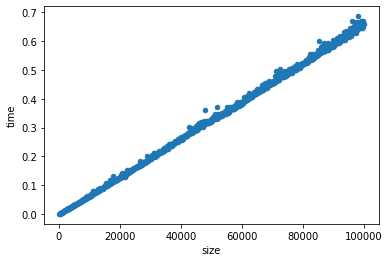
\includegraphics[width=0.95\textwidth]{h-size-time.png}
    \caption{Size - Time}
    \end{minipage}
    \begin{minipage}{0.48\textwidth}
    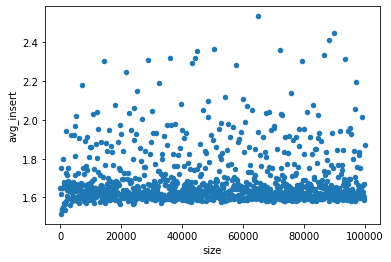
\includegraphics[width=0.95\textwidth]{h-size-insert.png}
    \caption{Size - Avg insert}
    \end{minipage}
    \begin{minipage}{0.48\textwidth}
    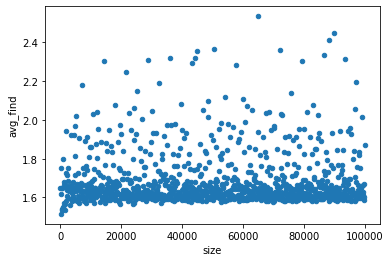
\includegraphics[width=0.95\textwidth]{h-size-find.png}
    \caption{Size - Avg find}
    \end{minipage}
\end{figure}

\subsection{Discussion}

Program runtime grows with the size of the data set and is almost proportional. This is logical because as the number of data increases, the time to complete all inserts and lookups increases in equal proportion.\\

\noindent The values of avg insert and avg distributed in a certain interval, there is no change in the range with data size. This trend is also seen in the collision rate, the percentage does not change with size. The operation cycle did not raize with the size of the data which means both insert and find operation can completed in a small number of cycles. This fits the O(1) although not perfectly. So the hypothesis that the time complexity of my algorithm is O(1) is satisfiable.\\

\noindent However the query hit rate in my test file is 100\%, which means everything that the program searched is in HashSet, there was no situation in the value was not fount in HashSet. This is a reason why operation cycles did not increase.


\section{Experiment 2}

In this experiment, the binary search tree will be used.

\subsection{Hypothesis}

The time complexity of binary search tree algorithm is O(h) where h is the height of the tree.

This means when the height increase, the time complexity will proportionally increase.

\subsection{Design}

\subsection{Results}

\subsection{Discussion}

\section{Conclusion}

\section{Experiment 3}

\appendix

%% And raw data or code scripts you want to present should be included as appendices.

\end{document}


